\documentclass[letterpaper,10pt]{article}

\usepackage{enumitem}
\usepackage{titling}
\usepackage{listings,listings-rust}
\usepackage{url}
\usepackage{soul}
\usepackage{hyperref}
\usepackage{setspace}
\usepackage{subfig}
\usepackage{sectsty}
\usepackage{pdfpages}
\usepackage{colortbl}
\usepackage{multirow}
\usepackage{multicol}
\usepackage{relsize}
\usepackage{amsmath}
\usepackage{wasysym}
\usepackage{fancyvrb}
\usepackage[yyyymmdd]{datetime}
\usepackage{amsmath,amssymb,amsthm,graphicx,xspace}
\usepackage[titlenotnumbered,noend,noline]{algorithm2e}
\usepackage[compact]{titlesec}
\usepackage{XCharter}
\usepackage[T1]{fontenc}
\usepackage[scaled]{beramono}
\usepackage[normalem]{ulem}
\usepackage{booktabs}
\usepackage{tikz}
\usetikzlibrary{arrows.meta,automata,shapes,trees,matrix,chains,scopes,positioning,calc,decorations.pathreplacing}
\tikzstyle{block} = [rectangle, draw, fill=blue!20, 
    text width=2.5em, text centered, rounded corners, minimum height=2em]
\tikzstyle{bw} = [rectangle, draw, fill=blue!20, 
    text width=4em, text centered, rounded corners, minimum height=2em]

\definecolor{namerow}{cmyk}{.40,.40,.40,.40}
\definecolor{namecol}{cmyk}{.40,.40,.40,.40}
\renewcommand{\dateseparator}{-}

\let\LaTeXtitle\title
\renewcommand{\title}[1]{\LaTeXtitle{\textsf{#1}}}

\lstset{basicstyle=\footnotesize\ttfamily,breaklines=true}

\newcommand{\CPP}{C\nolinebreak\hspace{-.05em}\raisebox{.4ex}{\tiny\bf +}\nolinebreak\hspace{-.10em}\raisebox{.4ex}{\tiny\bf +}}
\def\CPP{{C\nolinebreak[4]\hspace{-.05em}\raisebox{.4ex}{\tiny\bf ++}}}

\newcommand{\handout}[5]{
  \noindent
  \begin{center}
  \framebox{
    \vbox{
      \hbox to 5.78in { {\bf ECE459: Programming for Performance } \hfill #2 }
      \vspace{4mm}
      \hbox to 5.78in { {\Large \hfill #4  \hfill} }
      \vspace{2mm}
      \hbox to 5.78in { {\em #3 \hfill \today} }
    }
  }
  \end{center}
  \vspace*{4mm}
}

\newcommand{\lecture}[3]{\handout{#1}{#2}{#3}{Lecture#1}}
\newcommand{\tuple}[1]{\ensuremath{\left\langle #1 \right\rangle}\xspace}

\addtolength{\oddsidemargin}{-1.000in}
\addtolength{\evensidemargin}{-0.500in}
\addtolength{\textwidth}{2.0in}
\addtolength{\topmargin}{-1.000in}
\addtolength{\textheight}{1.75in}
\addtolength{\parskip}{\baselineskip}
\setlength{\parindent}{0in}
\renewcommand{\baselinestretch}{1.5}
\newcommand{\term}{Winter 2020}

\singlespace


\begin{document}

\lecture{29 --- Clusters \& Cloud Computing}{\term}{Patrick Lam}

\section*{Clusters and cloud computing}
Almost everything we've seen so far has improved performance on a single
computer. Sometimes, you need more performance than you can get on a
single computer. If you're lucky, then the problem can be divided
among multiple computers. We'll survey techniques for programming for
performance using multiple computers; although there's overlap with
distributed systems, we're looking more at calculations here.

\subsection*{Message Passing} For the majority of this course, 
we've talked about shared-memory systems. Last week's discussion of
GPU programming moved away from that a bit: we had to explicitly
manage copying of data. Message-passing is yet another paradigm.  In
this paradigm, often we run the same code on a number of nodes. These
nodes may potentially run on different computers (a cluster),
which communicate over a network.

MPI, the \emph{Message Passing Interface}, is a de facto standard for
programming message-passing systems. Communication is explicit in MPI:
processes pass data to each other using {\tt MPI\_Send} and {\tt
  MPI\_Recv} calls. 

Relevant piece about the relevance of MPI today:~\cite{hpcmpi}

\paragraph{Hello, World in MPI.} As with OpenCL kernels,
the first thing to do when writing an MPI program is to
figure out what the current process is supposed to compute.
Here's fairly standard skeleton code for that,
from \url{http://www.dartmouth.edu/~rc/classes/intro_mpi/}:

{\small
\begin{lstlisting}[language=C]
#include <stdio.h>
#include <mpi.h>

int main (int argc, char * argv[])
{
  int rank, size;

  MPI_Init (&argc, &argv);	/* starts MPI */
  MPI_Comm_rank (MPI_COMM_WORLD, &rank);	/* get current process id */
  MPI_Comm_size (MPI_COMM_WORLD, &size);	/* get number of processes */
  printf( "Hello world from process %d of %d\n", rank, size );
  MPI_Finalize();
  return 0;
}
\end{lstlisting}
}

\paragraph{Simple communication example.} The slides and live coding example contain
a second MPI example which demonstrates {\tt MPI\_Send} and  {\tt MPI\_Recv} usage,
also found at \url{http://en.wikipedia.org/wiki/Message_Passing_Interface}.

\paragraph{Matrix multiplication example.} We'll next discuss the code 
from another MPI example. You can find the code at
\url{http://www.nccs.gov/wp-content/training/mpi-examples/C/matmul.c}.
I'll discuss the structure of the code and
include relevant excerpts. Here are the steps that the program uses
to compute the matrix product $AB$:

\begin{enumerate}
\item Initialize MPI, as in the Hello, World example.
\item If the current process is the master task (task id 0):
\begin{enumerate}
\item Initialize the matrices.
\item Send work to each worker task: row number (offset); number of rows;
row contents from $A$; complete contents of matrix $B$. For example,

{\scriptsize
\begin{verbatim}
MPI_Send(&a[offset][0], rows*NCA, MPI_DOUBLE, dest, mtype, MPI_COMM_WORLD);
\end{verbatim}
}

\item Wait for results from all worker tasks (\verb+MPI_Recv+).
\item Print results.
\end{enumerate}
\item For all other tasks:
\begin{enumerate}
\item Receive offset, number of rows, partial matrix $A$, and complete matrix $B$, using {\tt MPI\_Recv}, e.g.

{\scriptsize
\begin{verbatim}
MPI_Recv(&offset, 1, MPI_INT, MASTER, mtype, MPI_COMM_WORLD, &status);
\end{verbatim}
}
\item Do the computation.
\item Send the results back to the sender.
\end{enumerate}
\end{enumerate}

\paragraph{On communication complexity.} To write fast MPI programs,
keeping communication complexity down is key. Each step from multicore
machines to GPU programming to MPI brings with it an
order-of-magnitude decrease in communication bandwidth and a similar
increase in latency.

\subsection*{Cloud Computing}
Historically, if you wanted a cluster, you had to find a bunch of
money to buy and maintain a pile of expensive machines. Not anymore.
Cloud computing is perhaps way overhyped, but we can talk about 
one particular aspect of it, as exemplified by Amazon's Elastic
Compute Cloud (EC2).

Consider the following evolution:
\begin{itemize}
\item Once upon a time, if you wanted a dedicated server on the
  Internet, you had to get a physical machine hosted, usually in a
  rack somewhere. Or you could live with inferior shared hosting.
\item Virtualization meant that you could instead pay for part of a
  machine on that rack, e.g. as provided by {\tt slicehost.com}.  This
  is a win because you're usually not maxing out a computer, and you'd
  be perfectly happy to share it with others, as long as there are
  good security guarantees. All of the users can get root access.
\item Clouds enable you to add more machines on-demand. Instead of
  having just one virtual server, you can spin up dozens (or
  thousands) of server images when you need more compute
  capacity. These servers typically share persistent storage, also in
  the cloud. 
\end{itemize}

In cloud computing, you pay according to the number of machines, or
instances, that you've started up. Providers offer different instance
sizes, where the sizes vary according to the number of cores, local
storage, and memory. Some instances even have GPUs, but it seemed 
uneconomic to use this for Assignment 3. Instead we have the {\tt ecetesla} machines.

\paragraph{Launching Instances.} When you need more compute power,
you launch an instance. The input is a virtual machine image.  You use
a command-line or web-based tool to launch the instance.  After you've
launched the instance, it gets an IP address and is
network-accessible. You have full root access to that instance.

Amazon provides public images which run a variety of operating
systems, including different Linux distributions, Windows Server, and
OpenSolaris. You can build an image which contains the software you
want, including Hadoop and OpenMPI.

\paragraph{Terminating Instances.} A key part of cloud computing is
that, once you no longer need an instance, you can just shut it down
and stop paying for it. All of the data on that instance goes away.

\paragraph{Storing Data.} You probably want to keep some persistent results
from your instances. Basically, you can either mount a storage device,
also on the cloud (e.g. Amazon Elastic Block Storage); or, you can
connect to a database on a persistent server (e.g. Amazon SimpleDB or
Relational Database Service); or, you can store files on the Web
(e.g. Amazon S3). 


\section*{Clusters versus Laptops}
There is a paper about this: Frank McSherry, Michael Isard, Derek G. Murray. ``Scalability! But at what COST?'' HotOS XV. This part of the lecture is based on the companion blog post~\cite{scalecost}.

The key idea: scaling to big data systems introduces substantial overhead. Let's just see how, say, a laptop compares, in absolute times, to 128-core big data systems.

\paragraph{Summary.} Big data systems haven't yet been shown to be obviously good; current evaluation is lacking.
The important metric is not just scalability; absolute
performance matters a lot too. We don't want a situation where we are just scaling up to $n$ systems to deal with the complexity of scaling up to $n$ systems. Or, as Oscar Wilde put it: ``The bureaucracy is expanding to meet the needs of the expanding bureaucracy.''

\paragraph{Methodology.} We'll compare a competent single-threaded implementation to top
big data systems, as described in an OSDI 2014 (top OS conference) paper on GraphX\cite{graphx}. The domain: graph processing
algorithms, namely PageRank and graph connectivity (for which the bottleneck is label propagation). The subjects: graphs with billions of edges, amounting to a few
GB of data.

\paragraph{Results.} 128 cores don't consistently beat a laptop at PageRank: e.g. 249--857s on the twitter\_rv dataset for the big data system vs 300s for the laptop, and they are 2$\times$ slower for label
propagation, at 251--1784s for the big data system vs 153s on
twitter\_rv. From the blogpost:

\begin{center}
	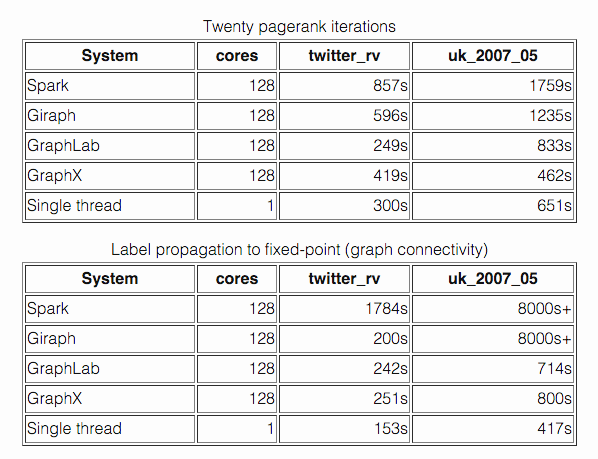
\includegraphics[width=0.60\textwidth]{images/pagerank.png}
\end{center}

\paragraph{Wait, there's more.} I keep on saying that we can improve algorithms for additional performance boosts too.
But that doesn't generalize, so it's hard to teach. In this case, two improvements are: using Hilbert curves
for data layout, improving memory locality, which helps a lot for PageRank; and using a union-find algorithm 
(which is also parallelizable). ``10$\times$ faster, 100$\times$ less embarrassing''.  We observe an overall
$2\times$ speedup for PageRank and $10\times$ speedup for label propagation.

\paragraph{Takeaways.} Some thoughts to keep in mind, from the authors:
\begin{itemize}
\item    ``If you are going to use a big data system for yourself, see if it is faster than your laptop.''
\item    ``If you are going to build a big data system for others, see that it is faster than my laptop.''
\end{itemize}



\section*{Movie Hour}
Let's take a humorous look at cloud computing: James Mickens' session from Monitorama PDX 2014. 

\begin{center}
\url{https://vimeo.com/95066828}
\end{center}

\bibliographystyle{alphaurl}
\bibliography{459}


\end{document}
